\chapter{心肺脑复苏}

\section{前沿学术综述}

针对心跳呼吸骤停采取的抢救措施称为心肺复苏(cardiac pulmonary
resuscitation,CPR)。随着CPR技术的进步,许多心跳呼吸骤停的患者能够恢复自主呼吸和循环,而脑功能恢复却成为影响预后的严重障碍,进而提出心肺脑复苏(cardiac
pulmonary cerebral
resuscitation,CPCR)的概念,旨在强调脑保护和脑复苏在抢救心跳呼吸骤停过程中的重要性。目前多数文献中CPR和CPCR是通用的。

现代CPR的基本框架形成于20世纪50年代至60年代,其标志是确立了CPR的四大基本技术,即口对口人工呼吸、胸外心脏按压、体表电除颤和肾上腺素等药物的应用。经过近半个世纪的发展,CPR技术日臻完善。欧美等国家多次召集全球性CPR专题会议,颁布和多次修订各自的心肺复苏标准或《指南》。在此基础上,国际复苏联络委员会(international
liaison committee on
resuscitation)于2000年颁布了第一部国际性复苏《指南》,即《国际心肺复苏和心血管急救指南2000》。此后,国际复苏联络委员会相继召开一系列会议,不断总结复苏医学领域的研究成果,并对新的临床证据进行科学评估。继2005年《指南》修订后,又于2010年9月和10月相继发表美国心脏病学会(AHA)的《2010
AHA心肺复苏与心血管急救指南》和国际复苏联络委员会的《2010心肺复苏和心血管急症科学及治疗建议的协调意见》
\protect\hyperlink{text00023.htmlux5cux23ch1-22}{\textsuperscript{{[}1{]}}}
\textsuperscript{,}
\protect\hyperlink{text00023.htmlux5cux23ch2-22}{\textsuperscript{{[}2{]}}}
。新《指南》的主要修订有以下几方面。

\subsubsection{复苏顺序}

2005年及之前的指南规定成人和儿童进行基本生命支持时,心跳呼吸骤停的复苏顺序为开放气道→急救呼吸→胸外按压,2010年新《指南》修订,建议复苏顺序改为胸外按压→开放气道→急救呼吸,即由ABC改为CAB。新指南极为强调高质量胸外按压的重要性,从基本生命支持流程中去除看、听和感觉等判断心搏骤停的步骤,主张一旦发现患者无反应和无呼吸(或无正常呼吸),应立即进行快速和有力的胸外按压。鼓励路人施救者无法或不愿意实施口对口急救通气时,也务必提供无通气的胸外按压。若能够提供急救呼吸,则以30∶2的按压通气比进行。

但对于专业抢救人员,复苏顺序的选择应根据可能的心脏停跳原因而有所不同。例如,若判定患者为溺水或其他可能的窒息性心脏停跳,则在激活急救反应系统前,先进行2次急救呼吸,紧接着按30∶2的比例给予5个周期(约2分钟)的CPR。而新生儿的停搏更可能是呼吸原因,应该以ABC顺序进行复苏,除非已明确为心脏原因导致的心跳骤停。

\subsubsection{高级生命支持阶段的监测和治疗}

在高级生命支持阶段,2010指南建议对气管插管的心跳骤停患者进行连续的定量二氧化碳波形图监测,以便证实气管导管的正确位置,监测心肺复苏质量,并辅助及时识别自主循环的恢复。新《指南》对传统高级生命支持流程图进行了简化和修改,新制定的环形抢救流程图更强调高质量CPR的重要性
\protect\hyperlink{text00023.htmlux5cux23ch3-22}{\textsuperscript{{[}3{]}}}
。在药物处理时,提出腺苷可用于稳定型无差异节律单一形态QRS复合波心动过速的治疗。

\subsubsection{心搏骤停后处理}

新指南增加了一个心跳骤停后处理(post-cardiac arrest
care)独立章节,建议对于心搏骤停后自主循环恢复而入院的患者,应该始终如一贯彻全面、有组织、完整和多学科协作的停搏后处理体系,以最终改善患者的预后。主张针对心跳骤停后综合征的处理应开始于心搏骤停的识别,持续到自主循环恢复,乃至出院及其以后阶段。极为强调多学科合作的综合性系统处理的重要性。

\section{临床问题}

\subsection{心跳骤停的判断和心肺复苏基本步骤}

\subsubsection{心肺复苏包括哪几个阶段?}

传统上,心肺复苏包括基本生命支持(basic life
support)、高级生命支持(advanced life
support)和复苏后处理(post-resuscitation care)3个阶段。

(1)基本生命支持 指心跳骤停发生后就地进行的抢救,基本目的是在尽可能短的时间里进行有效的人工循环和人工呼吸,为心脑提供最低限度的血流灌注和氧供。基本生命支持抢救现场可能在医院内,更多的可能在医院外,故相当多的施救者可能是非专业人员,而且此阶段大多在没有任何设备的情况下进行,即所谓的徒手心肺复苏。

(2)高级生命支持 指由专业医务人员在心跳呼吸停止的现场,或在向医疗单位转送途中进行的抢救。此阶段已有可能借助一些仪器设备和药品实施更有效的抢救,例如进行电击除颤、建立人工气道和人工通气、开通静脉通路和应用复苏药物等。

(3)心跳骤停后处理 2010年指南提出心跳骤停后处理(post-cardiac arrest
care)的新概念,更强调多学科合作的有机整合性综合处理的重要性。心跳骤停后处理指自主循环恢复后在重症医学科等实施的进一步治疗措施,主要包括以脑复苏或脑保护为核心的全身支持和治疗。治疗方案中应包括低温疗法、优化的目标指向性血流动力学监测和治疗、呼吸治疗、抽搐/肌阵挛控制、血糖控制,以及针对肺栓塞及急性冠状动脉综合征的多学科处理等。

\subsubsection{何谓心跳骤停的存活链?}

心跳骤停的存活链(chain of
survival)是指抢救心跳骤停的几个关键步骤。只有各步骤紧密衔接,环环相扣,才可能提高存活率。2010年指南增加了第5环。根据最新的描述,院外心跳骤停的存活链是:①立即识别心跳骤停和激活急救反应系统;②及早进行胸外按压为重点的心肺复苏;③迅速电除颤;④有效的进一步生命支持;⑤整体化的心跳骤停后处理。

\begin{center}
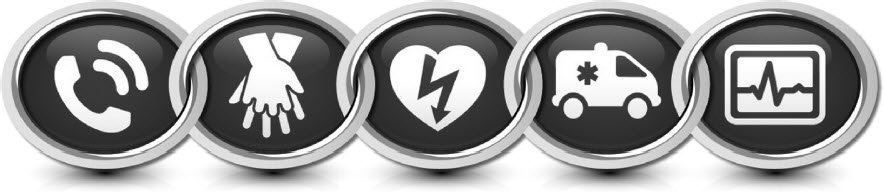
\includegraphics{./images/Image00136.jpg}
\end{center}

\subsubsection{心跳骤停的心电图类型有哪些?}

心跳骤停的心电图类型包括心室颤动、无脉搏性室性心动过速、心室停顿和无脉搏电活动(pulseless
electrical
activity)等几种,依据是否需要进行电击除颤及电击是否能够有效恢复灌注性心律,又分为可电击性心律(shockable
rhythms)和非可电击性心律(non-shockable rhythms)两类。

可电击性心律包括心室颤动和无脉搏室性心动过速,其发病率最高,抢救成功率也最高,故受到高度重视。抢救成功的关键在于及早电击除颤和及时有效的心肺复苏。非可电击性心律指心室停顿和无脉搏电活动。无脉搏电活动涵盖一组不同的无脉搏心律:假性电机械分离、心室自主节律、心室逸搏节律及除颤后心室自主节律等,复苏效果普遍极差。处理两组心律失常的主要区别在于前者需要进行电除颤。其他抢救措施包括胸外按压、气道管理和通气、静脉通路建立、应用肾上腺素及纠正可逆性病因等均相同。

\subsubsection{心跳骤停的常见原因有哪些?}

除心脏本身的病变外,休克、缺氧、严重水电解质平衡和代谢紊乱、中毒和呼吸系统疾病等均可导致心跳骤停,现场抢救时若能及时判断诱发心脏停跳的原因,并及时予以纠正,可能有利于自主循环的恢复。为方便记忆,可按“6H5T”的提示分析停跳原因。

\begin{table}[htbp]
\centering
\caption{心跳骤停的常见原因}
\label{tab17-1}
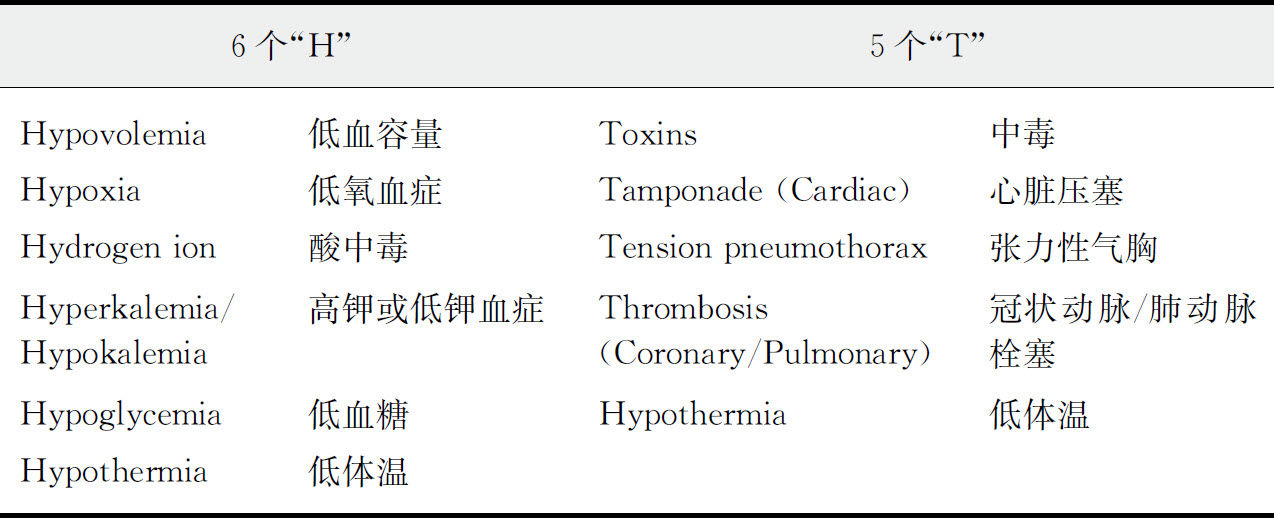
\includegraphics{./images/Image00137.jpg}
\end{table}

\subsubsection{如何判断呼吸心跳骤停?}

心跳呼吸停止的判断越迅速越好,只需进行患者有无应答反应、有无呼吸及有无心跳三方面的判断。院内急救可能略有区别(如监测下的心跳骤停),但也应避免不必要的延误,如找听诊器听心音、测量血压、连接心电图、检查瞳孔等。

(1)判断患者有无反应 循环停止10秒钟,大脑因缺氧而发生昏迷,故意识消失是心跳骤停的首要表现。判断意识消失的方法是拍打或摇动患者,并大声呼唤。

(2)判断有无呼吸 心跳停止者大多呼吸停止,偶尔也可有叹息样或不规则呼吸,部分患者则有明显气道梗阻表现。判断的方法是,用眼睛观察患者胸廓有无隆起的同时,施救者将自己的耳面部靠近患者口鼻,感觉和倾听有无气息。判断时间不应超过10秒钟。若不能肯定,应视为呼吸不正常,立即采取复苏措施。

(3)判断有无心跳 徒手判断心跳停止的方法是触觉颈总动脉搏动,首先用示指和中指触摸到甲状软骨,再向外侧滑到甲状旁沟即可。脉搏检查也应在10秒钟内完成。

2010年指南简化了基本生命支持程序,删除了“看、听和感觉”步骤。近年的研究证实,这些检查步骤的敏感性和特异性均不佳,完成这些步骤不但无助于准确判断心跳呼吸骤停,反而耗费时间而延误抢救,故强调对无意识、无呼吸或无正常呼吸(如仅有叹气样呼吸)的成人患者,应迅速激活急救反应系统,即刻进行以胸外按压开始的CPR。

\subsubsection{复苏顺序由ABC改为CAB}

即由开放气道→急救呼吸→胸外按压,改变为胸外按压→开放气道→急救呼吸。此修订旨在尽可能缩短停跳至首次胸外按压的时间。因胸外按压可立即实施,而进行急救呼吸前需要调整患者头部位置、密封气道进行口对口人工呼吸,或装配呼吸球囊面罩,均耗费时间而延迟启动心肺复苏(CPR)。开始复苏时立即给予30次胸外按压而不是两次通气,可减少首次按压的延迟。

对于专业抢救人员,复苏顺序的选择应根据可能的停跳原因而有所不同。例如,若判定患者为溺水或其他可能的窒息性心脏停跳,则在激活急救反应系统前,先进行2次急救呼吸,紧接着按30∶2的比例给予5个周期(约2分钟)的CPR
\protect\hyperlink{text00023.htmlux5cux23ch4-22}{\textsuperscript{{[}4{]}}}
。而新生儿的停搏更可能是呼吸原因,仍应以ABC顺序进行复苏,除非已明确为心脏原因导致的心脏骤停。

\subsubsection{胸外心脏按压-人工通气比例的选择}

2000年《指南》曾建议,胸外心脏按压的频率为100次/分,按压-人工通气比为15∶2。可以肯定,由于心肺复苏(CPR)时肺血流量减少,以远低于正常的频率进行通气,便足以维持肺的通气/血流比值。数学计算和动物模型均显示,减少通气次数,以高于15∶2的按压-通气比进行CPR,有可能使肺的通气/血流比更为匹配。对于发病率最高的室颤心跳骤停复苏而言,在停跳后的第一分钟里,进行有效的胸外心脏按压比人工通气更为重要。

近年来的临床研究发现,无论是专业急救人员还是路人所提供的CPR均有缺陷,主要表现为胸外按压的频率慢和深度不够,按压的中断过于频繁和时间过长,而同时普遍存在人工通气过度的现象。资料显示,路人给予2次急救呼吸所需要的时间长达14~16秒,而此时是无心脏按压的。动物实验也提示,频繁和长时间的胸外按压中断极为有害。胸外按压频繁中断和过度通气的结果,是心输出量减少、胸内压升高、冠状动脉灌注压和脑灌注压降低,从而导致复苏成功的可能性显著降低。

为了获得最优化的按压-通气比和尽量减少按压的中断,经过专家充分协商后建议,单人施救时统一采用30∶2的按压通气比,这一比例适用于从小儿(新生儿除外)到成人的所有心跳骤停患者。对所有非医务人员(路人)进行CPR培训时,无论单人或双人施救,均简化为30∶2。考虑到小儿发生心跳骤停更多系窒息原因所致,对婴儿及青春期前儿童患者实施双人CPR时,可采用15∶2比例,这里施救者应当为专业健康工作者和救护员。而对于新生儿,氧合和通气至关重要,故仍保留3∶1的按压-通气比。

专家鼓励施救人员提高胸外心脏按压的质量,即按压用力和快速,按压放松时让胸壁充分回弹,并尽可能减少按压中断。施救者进行这样的按压几分钟后就可能疲劳,从而按压和胸壁放松的质量下降,故有多名施救者时应尽可能轮换进行(约2分钟轮换1次,轮换时进行心律检查)。

\subsection{气道开放和人工呼吸}

\subsubsection{如何进行徒手开放气道?}

心跳骤停后昏迷的患者,舌根、软腭及会厌等口咽软组织松弛后坠,必然导致上呼吸道梗阻。解除上呼吸道梗阻的基本手法有3种:仰头法、抬颏法和托颌法。仰头抬颏常常结合使用。

(1)仰头抬颏法 施救者一手置于患者额头,轻轻使其头部后仰,另一手置于其颏下,轻轻抬起使颈部前伸。

(2)托颌法 施救者的示指及其他手指置于下颌角后方,向上和向前用力托起,并利用拇指轻轻向前推动颏部使口张开。

绝大多数口腔软组织导致的气道梗阻,通过以上手法便可解除。效果不佳时,应查找其他导致梗阻的原因。若口腔内可见固体异物,应立即用手指清除。患者若戴有假牙,已经破损或不能恰当固位者,应该取出,但固定良好的完好假牙可保留,以维持口腔的整体外形,便于面罩加压通气时的有效密闭。

\subsubsection{怀疑颈椎损伤者如何进行徒手开放气道?}

对怀疑存在颈椎损伤(如高处坠落伤、头颈部创伤、浅池跳水受伤等)患者复苏时,应保持患者的头、颈、胸和腰等部位处在自然位置。过度仰头可能加重颈髓损伤。一般仅采用托颌法开放气道,并由助手用手保持头和颈稳定在一条直线的位置。如果气道梗阻危及生命,即使采取正确的托颌法也不能解除时,可略微使头部后仰至气道开放。此时建立通畅呼吸道应该优先于预防潜在颈椎损伤。

\subsubsection{如何利用辅助器械进行气道开放?}

常用于气道开放的辅助器械分为基本气道设备和高级气道设备两种。

基本气道开放设备指口咽通气道和鼻咽通气道,分别经口和鼻孔放置,深入到咽部,将后坠的舌根等软组织推开,从而解除梗阻。怀疑颅底骨折时,应避免选用鼻咽通气道。

高级气道设备包括气管内导管、食管气管联合导管(combitube)和喉罩(laryngeal
mask)3种。一般认为,气管内导管是心跳骤停时管理气道的最佳方法,后两者也可作为有效的替代措施。但进行气管插管等操作时必须中断胸外按压,应尽可能缩短按压中断时间。为避免在复苏早期有长时间的胸外按压中断,有人主张自主循环恢复后再进行气管内插管。究竟选用何种方法,取决于心跳骤停现场的条件,以及施救者的经验和能力。放置高级气道后不仅能够保障气道开放,尚可连接呼吸机或呼吸囊进行人工通气。此时人工通气可以8~10次/分钟的固定频率进行,不考虑通气与按压的比例,也不得中断胸外按压。

\subsubsection{如何进行口对口和口对鼻人工呼吸?}

口对口人工通气是心肺复苏的基本技术之一。正常人呼出气的氧浓度为16%~17%,尽管如此,吹入心跳呼吸停止患者的呼吸道,仍可有效缓解严重缺氧。进行口对口通气时,施救者一手捏住患者鼻子,另一手推起患者颏部保持气道开放,眼睛观察胸部运动。平静吸气(不必深吸气)后,用口包住患者口腔向里吹气。吹气时间大约1秒,观察到胸部隆起即可。有时须采用口对鼻通气做为口对口通气的替代方法,如对口腔严重创伤而不能张开者、口对口通气无法密闭者、或溺水者在水中施救等。唯吹气时应将口唇捏住,其他要求与口对口通气一致。

\subsubsection{如何应用气囊-面罩进行人工通气?}

院内心肺复苏时一般用气囊-面罩进行人工通气。目前普遍应用的自充式气囊不接氧气时也可提供氧浓度为21%的气体,接氧气后氧浓度可达到45%;若带有储气囊,氧流量为10L/分钟时,可使吸氧浓度提高到85%。单人进行气囊-面罩通气时,施救者一只手用拇指和示指扣压面罩,中指及其他手指抬起下颌,另一只手捏气囊,技术要求颇高,且容易疲劳。双人操作则容易保障有效的开放气道和通气。无论单人还是双人操作,通气量只需使胸廓隆起即可,频率保持在8~10次/分钟,避免快速和过分用力加压通气。

\subsubsection{心肺复苏时呼气末二氧化碳波形监测有何意义?}

呼气末二氧化碳系通过串联在气管导管上的二氧化碳探头,描计呼出和吸入气体中的二氧化碳浓度波形。心脏停跳时全身循环停止,组织中的二氧化碳不能被有效清除,呼出气中的二氧化碳水平低下;只有在有效循环灌注前提下(无论是人工循环还是自主循环),才可能在呼出气体中检测出高浓度的二氧化碳。2010《指南》建议,有条件时应对气管插管的心跳骤停患者进行连续呼气末二氧化碳监测。目的在于:①证实气管导管的正确位置(若导管误插入食管则无二氧化碳排出);②评估胸外按压的质量(呼气末二氧化碳水平低下提示所进行的胸外按压未能提供充分的组织血流灌注,从而使滞留于组织中的二氧化碳未能被清除出来);③判断有效自主循环的恢复(表现为呼气末二氧化碳水平骤然升高)。

\subsection{胸外按压和除颤}

\subsubsection{治疗室颤心跳骤停时,胸外心脏按压和电除颤的顺序是什么?}

电除颤是治疗室颤的有效手段已无庸置疑,但对所有室颤者均无例外地首先进行电除颤的做法受到挑战。研究显示,心跳骤停发生至急救人员到达现场并实施首次电除颤的时间,若超过4~5分钟或更长时,先进行一段时间的心肺复苏(CPR),然后再进行电除颤,能够提高存活率。但也有1项研究显示,先行CPR和先电除颤两种做法对于存活率的影响没有统计学差别。最后的协调意见是,目前尚缺乏充分证据建议对所有室颤停跳患者均首先进行CPR。2005年指南提出,对于院外室颤或无脉搏的室性心动过速,若急救人员到达时停跳已超过4~5分钟,或非急救人员目击下的停跳,可先进行5个30∶2周期(或大约2分钟)的CPR再实施电除颤
\protect\hyperlink{text00023.htmlux5cux23ch5-22}{\textsuperscript{{[}5{]}}}
。若同时有多个急救者到达现场,应有一人立即进行CPR,其他人准备除颤器并及早除颤
\protect\hyperlink{text00023.htmlux5cux23ch6-22}{\textsuperscript{{[}6{]}}}
。

\subsubsection{如何进行胸外按压?}

胸外按压通过提高胸腔内压力和直接压迫心脏而使血液流动。操作手法正确时,可使收缩(按压)压达到60~80mmHg,但舒张压依然低下,平均动脉压极少超过40mmHg。尽管如此,按压产生的血流可为心肌和脑组织提供一定水平的血流灌注,对于恢复自主循环和减轻脑缺氧损害至关重要。尤其在心脏停跳倒地时间超过5分钟的患者,有效胸外按压可增加电除颤成功的可能性。目前认为,高质量的胸外按压是复苏成功的关键,其要点如下:

(1)按压部位及定位 按压定位在胸骨下半部分的中间。过去曾建议,施救者定位时先用手指触摸到肋弓,滑向剑突,然后向上找到胸骨下段,手法烦琐费时,且无必要。2005年指南建议直接将手掌置于胸部中央相当于双乳头连线水平即可。2010《指南》简化为“将手掌置于胸部中央”即可。

(2)按压手法 施救者用一只手的掌根置于按压点,另一手掌重叠于其上,手指交叉并翘起;双肘关节与胸骨垂直,利用上身的重力快速下压胸壁。

(3)按压频率和深度 按压必须快速有力,频率至少为100次/分钟(2005年指南规定为接近100次/分钟),深度至少为5cm(2005年指南规定为4~5cm)。

(4)按压和放松时间 按压放松时间大致相当,放松时手掌不离开胸壁,但必须让胸廓充分回弹。

(5)按压/通气比 单人施救时统一为30∶2,适于对从小儿(除新生儿外)到成人的所有心脏停跳者进行心肺复苏(CPR)。因小儿停跳多系窒息所致,故专业急救人员对婴儿及青春期前儿童进行双人CPR时,可采用15∶2的按压-通气比;而新生儿CPR时,对氧合和通气的要求远远高于胸外按压,应保留3∶1按压-通气比。

(6)按压效果评价 不要依赖颈动脉或股动脉搏动来评估按压是否有效。为了保障高质量的胸外按压,除用力和快速按压以外,必须最大限度地减少按压中断的次数和时间。正确的胸外按压极易疲劳,多人施救应尽可能轮换进行,以免影响按压质量。一般约2分钟应轮换一次,可利用轮换时间进行心律检查。

\subsubsection{何谓单纯胸外按压心肺复苏?}

单纯胸外按压心肺复苏(Compression-only
CPR)指仅做胸外按压而不给予人工通气的心肺复苏(CPR)。大量调查证实,绝大部分专业医务人员和路人施救者,均不愿意为陌生的心跳骤停患者实施口对口通气。除普遍顾虑传染疾病外,患者口鼻处常常有出血或呕吐物,也必然使施救者产生心理上的障碍。

动物研究显示,在窒息性心脏停跳的最初数分钟内,仅仅进行胸外按压,可能与胸外按压加通气的复苏效果相当。如果气道开放良好,停跳后偶尔的喘气样呼吸和按压造成的胸廓被动运动,也可提供部分气体交换。由于胸外按压所能提供的心输出量低于正常,低分钟通气量可能足以使CPR期间的通气/血流灌注比匹配。近年来多个国家的一些观察性研究显示,对成人心跳骤停者施救时,单纯胸外按压的存活率优于无CPR,但最佳方式仍然是按压加通气CPR。

综合以上考虑,目前的建议是,鼓励未受过CPR训练、或不确定如何进行CPR者,可不做人工通气,但务必提供单纯按压的CPR。专业医务人员在院内施救时,应尽可能采用按压加通气的标准CPR。当然,若有可能,应充分利用面罩呼吸囊等辅助设备进行良好的人工通气。

\subsubsection{如何评价胸前捶击?}

心跳骤停后采用胸前捶击的理由是,捶击产生的机械性能量转化为电能,可能足以达到转律作用。目前,尚无前瞻性研究评估此方法的效果。一些病例总结报道胸前捶击可使室颤或无脉搏心动过速转变为灌注性心律,但胸前捶击成功终止心动过速的可能性最大,对室颤则效果不佳。所有报道胸前捶击成功除颤的病例均为心室颤动发生10秒钟以内者。另有报道,胸前捶击可能使心律恶化,如使心动过速加速,或者使心动过速转变为心室颤动、完全性传导阻滞或心室停顿。

目前建议,对于目击下心跳骤停患者,现场不能立即获得除颤器时,可考虑进行一次胸前捶击。这一般见于监测下的心跳骤停。此操作应由经过训练的医务人员进行,方法是用拳头尺侧从20cm高处快速捶击胸骨下半部分,并立即缩回,以产生一次冲击样刺激。

\subsubsection{为何要及早电击除颤?}

早期除颤是使患者心跳骤停后存活的关键,其理由如下:①目击下心跳骤停最常见的初始心律是室颤;②电击除颤是治疗室颤的有效手段;③除颤成功的可能性随时间推移而迅速降低(从患者倒地至首次电击的时间每延迟1分钟,死亡率增加7%~10%);④若不能及时终止室颤,有可能在数分钟内转变为心室停顿等更加难治的心律失常。

\subsubsection{除颤器的类型有哪些?}

除颤机理是以一定能量电流瞬间通过心肌,使绝大部分心肌细胞发生同步去极化,从而恢复窦性节律。目前用于心跳骤停抢救的除颤器均为非同步体表除颤器,有手动除颤器和自动体表除颤器(automated
external
defibrillators,AEDs)两大类,按所输出的除颤电流特征又可分为单相波除颤器和双相波除颤器。双相波除颤是近年来应用日益广泛的技术,其优点是除颤成功率高、除颤电能小,从而造成的心肌损害轻微,有取代单相波除颤的趋势。AEDs是专门为非急救专业人员设计的一种小型便携式除颤器,适用于公众场所或家庭,近年来也有主张在医院的普通医疗区域广泛配置。AEDs的使用极为简便,只有3个按键,在语音提示下依次按键操作即可,采用粘贴式电极片,可自动进行心电图检测,诊断是否为可电击性心律,以固定的电能进行双相波除颤,并可显示和自动记录心电图波形。

\subsubsection{如何进行电击除颤?}

(1)除颤适应证 电除颤治疗的适应证是室颤或无脉搏的室速(可电击性心律)。没有证据表明电除颤对治疗心室停顿等(非可电击性心律)有益,相反,重复电击可能导致心肌损害。目前除颤器一般具有快速监测和诊断功能,以确定是否存在室颤,不必要进行盲目除颤。

(2)除颤电极 除颤器的电极有手柄式和粘贴式两种,一般手动式除颤器多用手柄式电极,使用前需涂导电胶以减少与胸壁的电阻抗;自动体表除颤器多用粘贴式电极。两个电极并无左右正负之分,常用安放部位有:①胸骨心尖位(sternal-apical
position),是标准安放部位,应用最为广泛,电极置于胸骨右缘第2肋间和左第5肋间腋中线。②前后位,电极位置分别为左侧心前区和背部左肩胛骨下角处,一些自动体表除颤器的粘贴式电极常用此位置。③左右侧胸壁腋中线处,较少采用。

(3)除颤剂量(电击能量) 不同除颤仪和除颤波形所需要的电能不同,双相切角指数波用150J~200J,双相直线波用120J,单相波初始及后续电击均采用360J(先前建议由200J、300J到360J依次递增)。一般除颤器均在显著位置标明有效除颤电能,不了解所使用设备的有效剂量范围时,首次电击用200J,其后选用相同或更大剂量。若电击成功除颤后室颤复发,再次电击采用先前成功除颤的电能进行。

(4)电击前的心肺复苏 对倒地时间5分钟以上的患者,或所有非目击下的心跳骤停患者,均应先进行2分钟(5个30∶2周期)的心肺复苏,再进行电除颤。院内停跳一般发生于监测下或目击下,可考虑首先进行电除颤。

(5)电击次数 对所有室颤或无脉搏的室速电除颤治疗时,均采用单次电击策略。单次电除颤完毕立即恢复心肺复苏(CPR),首先进行胸外心脏按压,完成5个30∶2周期(或大约2分钟)的CPR后,再停止CPR检查循环状况(包括检查心律及脉搏)。

\subsection{心肺复苏的药物治疗}

\subsubsection{心肺复苏时如何选择给药途径?}

抢救心跳骤停的用药途径有3种:静脉途径、骨髓腔途径、气管途径,应优先采用静脉途径。静脉通路难以建立时,考虑采用后两种。

静脉途径又分为外周静脉和中心静脉两种。与外周静脉比较,经中心静脉用药血浆药物峰浓度高,循环时间短。但中心静脉置管操作需要中断心肺复苏(CPR),并且有许多并发症,而外周静脉置管快捷简便,一般作为首选。为了促进药物尽快进入中心循环,经外周静脉用药须在药物注射后推注20ml生理盐水,并抬高肢体10~20秒钟。

过去一般认为骨髓腔途径仅适用于无法建立血管通路的儿童患者,现已证明在成人也同样有效。经骨髓腔用药达到足够血浆浓度的时间与中心静脉相当。目前国外已有用于成人骨髓腔穿刺置管的套针上市。此外,骨髓腔途径也可以用于抽取骨髓进行血气分析、检测电解质和血红蛋白浓度等。

部分抢救药物可通过气管给药,但是通过气管给药所达到的血浆药物浓度难以准确预知,最佳用药剂量也不完全明确。已证明CPR时气管内应用肾上腺素的剂量是静脉用药剂量的3~10倍。故肾上腺素气管内给药时,单次剂量为3mg,用至少10ml的注射用水稀释后应用。已经证明,用注射用水稀释较生理盐水吸收更佳。

\subsubsection{肾上腺素仍然是心跳骤停的首选缩血管药吗?}

肾上腺素作为一种拟交感活性药物,应用于心跳骤停的抢救已有40余年,目前仍被推荐作为心跳骤停的标准缩血管药首选使用。其α肾上腺能受体活性导致体循环血管收缩,从而提高冠状动脉和脑灌注压,增加心脑血流量,有利于自主循环恢复和保护脑功能;其β受体兴奋引起的变力和变时作用,也有可能增加冠状动脉和脑血流量,但同时可增加心肌耗氧、诱发异位室性心律(尤其在酸中毒时)、增加肺动(静)脉分流导致一过性低氧血症等,从而抵消了其益处。

肾上腺素的用法是1mg静脉或骨髓腔内注射,每3~5分钟重复1次。若静脉通路未能及时建立,可通过气管导管使用肾上腺素,剂量为2~2.5mg。一般不推荐大剂量应用肾上腺素,特殊情况下考虑使用更高剂量(如β肾上腺受体阻滞剂或钙通道阻滞剂中毒等)。有时自主循环恢复后仍然需要用肾上腺素输注维持血压,应细心调节输注速率,以达到合适的血压水平,剂量过大可能导致心动过速和加重心肌缺血,并可能诱发室颤。对于可卡因或其他拟交感药物中毒导致心跳骤停的患者,使用肾上腺素应谨慎。

\subsubsection{怎样评价血管加压素在心肺复苏中的地位?}

血管加压素是天然的抗利尿激素,大剂量时刺激血管平滑肌上的V\textsubscript{1}
受体,产生强效缩血管作用。对院外心脏停跳患者血清血管加压素水平测定发现,成功复苏的患者血管加压素水平显著高于未复苏者,由此有人提出血管加压素可用于心跳骤停的抢救。临床和动物实验研究均表明,心跳骤停期间应用血管加压素替代肾上腺素,能够明显改善血流动力学。一些研究还提示应用血管加压素可以提高存活率,但目前没有足够证据支持将血管加压素常规作为心肺复苏的一线药物,或与肾上腺素联合使用。在1mg肾上腺素不能恢复自主循环时,可考虑应用血管加压素40U静脉推注。也可以用血管加压素40U代替首剂肾上腺素使用。血管加压素可能在心室停搏的治疗时更有效果。

\subsubsection{胺碘酮在心肺复苏中的作用如何?}

胺碘酮是作用于心肌细胞膜的抗心律失常药,通过对钠、钾和钙等离子通道的影响发挥作用。胺碘酮可延长心房和心室的心肌动作电位时程和不应期,延缓房室传导,并对旁路传导发挥类似作用。胺碘酮具有α和β肾上腺受体阻断活性,可产生轻度负性变力作用,并引起外周血管扩张。与安慰剂和利多卡因比较,胺碘酮应用于3次电击后仍持续心室颤动的患者,可提高入院存活率。用于人类或动物心室颤动或血流动力学不稳定的心动过速时,可能改善对电击除颤的反应。但目前的临床资料均为经过3次电击除颤,而心室颤动或心动过速持续存在的患者,尚无证据表明采用单次电击除颤策略后如何应用胺碘酮。

胺碘酮可用于对胸外按压、电击除颤和缩血管药等治疗无反应的心室颤动或无脉搏心动过速患者,初始剂量为300mg,用5%葡萄糖液稀释到20ml,静脉或骨髓腔内注射,随后可追加150mg。外周静脉注射胺碘酮可引起血栓性静脉炎,应尽可能从中心静脉导管给药。无中心静脉导管时,应选用大的外周静脉,给药后用液体推注。胺碘酮有时可诱发心律失常,尤其在与可能延长QT间期的药物同时使用后更易发生。但与其他抗心律失常药比较,相同情况下促进心律失常的发生率更低。其主要的急性副作用为低血压和心动过缓,缓慢静脉推注可预防急性副作用,必要时采取快速输液及正性肌力药等方法纠正。

\subsubsection{心肺复苏中推荐应用利多卡因吗?}

利多卡因是一种传统的抗心律失常药,通过稳定细胞膜,延长心肌细胞的不应期,降低心室肌的自主节律性,其局部麻醉作用则使心室异位节律活性减弱。

利多卡因抑制去极化的异位节律组织活性,而对正常心肌组织的电活动干预极小,故能够有效抑制与去极化相关的心律失常(如缺血、洋地黄中毒等),而对发生于正常极化细胞的心律失常相对无效(如心房颤动或心房扑动等)。利多卡因还可提高室颤的发生阈值。

利多卡因经过多年临床使用,是一种相对安全的抗心律失常药,但用于心跳骤停的治疗,其短期或长期效果均没有得到证实。近年来的研究发现,利多卡因用于心跳骤停,自主循环恢复率低于胺碘酮,而心室停顿的发生率高于后者,故目前仅推荐在没有胺碘酮时应用利多卡因抢救心跳骤停。顽固性心室颤动或心动过速而无胺碘酮可使用时,可考虑静脉推注利多卡因100mg(1~1.5mg/kg)。若心室颤动或心动过速持续存在,可每隔5~10分钟追加0.5~0.75mg/kg,第1小时的总剂量不超过3mg/kg。

利多卡因的毒性反应包括感觉异常、嗜睡、迟钝、肌肉抽搐和痉挛等,如果出现中毒表现,应立即停止输注。利多卡因抑制心肌功能,但是远较胺碘酮为轻,且通常是短暂的,可静脉应用缩血管药予以纠正。利多卡因在低钾血症和低镁血症时效果不佳,应注意及时纠正这些电解质紊乱。

\subsubsection{怎样认识静脉补充硫酸镁在心肺复苏中的重要性?}

镁是多种酶系统的重要组成部分,尤其在一些与肌肉ATP生成有关的酶类。镁离子在神经的化学传递方面也有重要作用,可减少乙酰胆碱释放,降低运动终板的敏感性。低镁血症常常与低钾血症相联系,可能是引起心律失常和心跳骤停的原因。镁缺乏时心肌对洋地黄类药物的摄取增加,并降低细胞Na+/K+-ATP酶的活性,故低镁血症和低钾血症的患者即使应用治疗剂量的洋地黄,也可能导致中毒。镁缺乏在临床并不少见,除低钾血症外,还常常伴有其他电解质紊乱,如低磷血症、低钠血症和低钙血症等。

已知镁缺乏时补充镁剂是有益的,但心跳骤停时常规使用镁剂的价值没有得到肯定。对院外成人心跳骤停患者的研究,也未证实心肺复苏时常规应用镁剂能够增加自主循环恢复。有一些证据显示,顽固性心室颤动时应用镁剂有益。镁剂使用的指征包括:①对电击无效的顽固性心室颤动,并可能有低镁血症;②室性心动过速并可能伴有低镁血症;③尖端扭转型室性心动过速;④洋地黄中毒。

对电击无效的顽固性心室颤动,静脉推注硫酸镁的初始剂量为2g(8mmol),1~2分钟注射完毕,10~15分钟后可酌情重复。镁离子抑制血管平滑肌收缩,引起血管扩张和与剂量相关的低血压,通常时间短暂,对输液和缩血管药等治疗反应良好。

\subsubsection{心肺复苏中阿托品的地位如何?}

阿托品是M型胆碱能受体拮抗剂,可阻断迷走神经对窦房结和房室结的作用,增加窦房结自主节律性,促进房室结传导。曾有应用阿托品后成功治疗心室停顿等的报道,但是新的研究证据显示无脉搏电活动或心室停顿时使用阿托品并无治疗益处,故2010年指南已不再建议阿托品常规用于此类患者。

但是,阿托品仍然是有症状性急性心动过缓的一线用药。成人研究表明,静脉注射硫酸阿托品可逆转胆碱能介导的心率过缓,对于有症状的窦性心动过缓、房室结水平的传导阻滞或窦性停搏患者,可有效加快心率、改善症状和体征。治疗心动过缓的建议剂量是静脉注射0.5mg,可每3~5分钟重复一次,最大剂量为3mg。急性冠状动脉缺血或心肌梗死时应用阿托品应谨慎,因为心率加快有可能加重心肌缺血和增加梗死面积。以下情形不宜应用阿托品:Ⅱ型Ⅱ度或Ⅲ度房室传导阻滞、Ⅲ度房室传导阻滞新发生宽QRS波患者。此时阻滞部位位于非结性组织(如希氏束或更远的传导组织),对阿托品的乙酰胆碱能逆转作用不会有反应,采用起搏器或β肾上腺能激动剂治疗效果更佳。

\subsubsection{心肺复苏中腺苷的地位如何?}

腺苷(adenosine)是一种内源性嘌呤核苷酸,可短时间抑制窦房结和房室结传导,并有血管扩张作用。2010年《指南》鉴于其安全性和潜在效果的新证据,推荐用于稳定型无差异节律的单一形态窄QRS波心动过速,或用于等待电转律的不稳定型窄QRS波节律整齐的心动过速,也可用于稳定型节律整齐的单一形态宽QRS波心动过速的治疗与诊断。用法是快速静脉注射6mg,随即推注20ml生理盐水,必要时重复静脉注射12mg。其副作用有低血压、支气管痉挛和胸前不适。哮喘的患者禁忌使用。另外,该药也有诱发快速性心房纤颤的可能性。

\subsubsection{心肺复苏中需要补充钙剂吗?}

钙离子在心肌细胞收缩机制中有重要作用,但是极少有资料支持心跳骤停后应用钙剂能够提供任何益处。注射钙剂后的高血钙对于缺血心肌和受损脑细胞的恢复反而可能有害。仅在一些特殊情况下需及时补钙:①高钾血症;②低钙血症;③钙离子通道阻滞剂中毒。初始使用剂量为10%氯化钙10ml(含钙离子6.8mmol)静脉推注,必要时可重复。静脉推注过快可减慢心律,导致心律失常,心跳骤停时可加快推注速度。须注意,不宜与碳酸氢钠经同一静脉通路同时补钙。

\subsubsection{碳酸氢钠在心肺复苏中需要常规补充吗?}

心跳骤停后可出现混合性酸中毒,既有呼吸性因素,又有代谢性因素。恢复酸碱平衡的最有效方法是通过良好的胸外按压以支持组织灌注和心输出量,争取迅速恢复自主循环,同时进行恰当的人工通气。

很少有资料支持心跳骤停期间应用碱剂治疗,反而有证据显示应用碳酸氢钠有许多副作用,其中包括:①轻度酸中毒可扩张脑血管而增加脑血流,完全纠正组织pH反而可能降低脑血流量;②所产生的二氧化碳能够自由弥散进入心肌和脑细胞,从而导致反常性的细胞内酸中毒、细胞外碱中毒;③产生高钠血症和高渗状态;④导致氧离解曲线左移,抑制组织的氧释放;⑤加重中心静脉酸中毒,可能使同时输入的儿茶酚胺类药物失效;⑥对缺血心肌产生负性肌力作用;⑦\ce{HCO3-}
最终以二氧化碳形式从肺部排除,使患者的通气负荷增加。

综上所述,只有严重代谢性酸中毒时才进行纠酸治疗,而在心跳骤停和胸外心脏按压(尤其院外停跳)期间,或自主循环恢复后阶段,均建议常规应用碳酸氢钠。复苏后动脉血气分析显示pH<7.1(BE在-10mmol/L以下)时可考虑应用碳酸氢钠。有以下情况时可考虑积极应用:①存在危及生命的高钾血症或高血钾引起的心脏停跳;②原有严重的代谢性酸中毒;③三环类抗抑郁药中毒。

应用碳酸氢钠的初始剂量为1mmol/kg静脉滴注,是否需要重复应根据血气分析的结果决定。也不必要完全纠正酸中毒,以免发生医源性碱中毒。高浓度的碳酸氢钠渗漏到皮下可引起严重组织损伤。

碳酸氢钠与钙离子结合可生成碳酸钙,故不应在同一通路中混合输入。

\subsubsection{如何评价心肺复苏期间的静脉输液?}

若心跳骤停与大量液体丧失导致的低血容量有关,应及时补液以迅速恢复血容量。对正常血容量的心跳骤停患者是否需要常规输液尚无临床研究的资料。实验性心室颤动动物的研究结果既不能支持也不拒绝常规静脉输液。无低血容量存在时,过量输注液体似乎并无益处。复苏期间建立静脉通路的主要目的是用药。除非明确存在低血糖,一般应避免输注含葡萄糖溶液。输注含糖液体容易引起高血糖,从而加重停跳后的神经功能障碍。

\subsection{心肺复苏后处理}

\subsubsection{自主循环恢复后如何进行呼吸支持?}

心跳停止时间短暂的患者,可能立即恢复正常脑功能,此类患者自主呼吸功能完善,不需要进行气管插管和机械通气,但短时间内应继续经面罩或鼻导管给氧。对复跳后存在任何程度脑功能障碍的患者,均应进行气管插管,以保障气道通畅及便于机械通气。已插管者应予保留,并检查导管位置是否正确。完全无自主呼吸或自主呼吸恢复不完善者应该实施机械通气。

近年研究显示,自主循环恢复后动脉高氧合状态,非但无益反而可能产生高氧损伤而增加病死率,故目前规定,在维持动脉血氧饱和度≥94%的前提下,尽量下调吸氧浓度。另有研究表明,心跳停止后过度通气可能不利于脑功能恢复。过度通气引起的低碳酸血症,可导致脑血管收缩,降低脑血流量,从而加重脑缺血;另外还可能使气道压力过高,增加内源性呼气末正压,使颅内静脉回流减少、颅内压升高、脑灌注减少。目前尚不能确定复苏后动脉血二氧化碳的目标水平。推荐的做法是通过呼气末二氧化碳监测和血气分析等指标调节机械通气参数,维持动脉血二氧化碳在正常水平(35~40mmHg)。

口对口或面罩加压通气可造成胃膨胀,从而限制膈肌运动及影响通气,为此可插胃管减压。剧烈咳嗽不但可使颅内压升高,并可能导致一过性低氧血症。对于呛咳反射活跃的患者,应给以充分的镇静。复苏后应该常规拍床旁胸部X线片,以便了解气管导管和中心静脉导管的位置、评估是否存在肺水肿,并排除肋骨骨折或气胸等胸外按压并发症。

\subsubsection{自主循环恢复后如何进行心血管功能支持?}

由于缺血再灌注损害和反复电击除颤的影响,自主循环恢复后可发生一过性的心肌功能障碍(心肌抑顿),导致血流动力学不稳定,表现为血压降低、心输出量减少及心律失常等。可持续数小时,但大多在24~48小时内恢复。此外,复苏后阶段血浆促炎性细胞因子水平显著升高,可出现类似于感染导致的全身性炎性反应综合征,表现为血管扩张性低血压,并有可能最终引发多器官功能障碍。有鉴于此,复苏后阶段早期大多需要应用缩血管药维持血压。并参考感染性休克的早期目标指向治疗策略,提供最优化的组织灌注和氧供。

复苏后应该加强血流动力学监测,一般应该进行动(静)脉穿刺置管以便监测有创动脉压和中心静脉压,必要时采用有创性或无创性心输出量检测可能更有帮助。依据监测结果,决定是增加输液量还是采用利尿、强心或扩血管药等措施。

目前尚无确切资料提示应将复苏后血压和血流动力学参数控制在何种水平,但有资料证明,自主循环恢复后最初2小时,平均动脉压水平高于100mmHg的患者,与低于100mmHg的患者比较,其神经系统功能恢复更佳。考虑到全脑缺血后可能发生脑水肿,需要更高的脑灌注压才能维持充分的脑血流,适当提高血压水平是合理的,至少不应低于患者平时的血压水平。

心律失常是心跳骤停的常见原因,但是复跳后预防性使用抗心律失常药是否有益尚无定论。短时间内继续应用与自主循环恢复有关的抗心律失常药可能是合理的。同样,考虑到β受体阻滞剂在缺血性心脏病中的心脏保护作用,复苏后如果没有禁忌证,可以使用β阻滞剂。

\subsubsection{如何进行自主循环恢复后的体温管理?}

自主循环恢复后的体温管理包括预防性治疗高热和治疗性低温疗法两方面。研究表明,体温在37℃以上均明显影响神经功能的恢复,故复苏后72小时内发生的高热均需积极处理。应采用药物或物理降温将体温控制在正常范围。

治疗性轻度低温疗法是指通过主动干预将患者体温控制在32~34℃水平,从而达到改善神经系统功能的恢复和增加存活率的目的。随机对照临床试验证实,对于初始心律为室颤的院外心脏停跳、自主循环复苏后仍处于昏迷状态的成人患者,数分钟或数小时内开始将其体温控制在32~34℃,持续12~24小时可以改善患者预后。还有证据显示,对初始心律为无脉搏电活动/心室停顿、复苏后仍昏迷的成人患者,实施轻度低温也能够改善代谢指标(血乳酸水平及氧摄取等)和神经学功能,而不增加并发症发生率
\protect\hyperlink{text00023.htmlux5cux23ch7-22}{\textsuperscript{{[}7{]}}}
。

(1)适应证 ①院外室颤性停跳、恢复自主循环后仍无意识(即对语言指令无反应者)的成人患者;②院外非可电击性停跳(无脉搏电活动/心室停顿)、复苏后仍昏迷的成人患者;③院内任何原因停跳、自主循环恢复后的昏迷患者。

心跳骤停后48小时内出现自发轻度低温的昏迷患者(>32℃),无需主动复温。

(2)目标温度和维持时间 控制中心体温(血液、膀胱、食管、外耳道、直肠或鼻腔等部位测量的温度)在32~34℃。降温开始时间越早越好,至少持续12~24小时。近年来有学者提倡维持至少72小时的轻度低温治疗,可能效果更佳。

(3)降温方法 有体表降温和内在降温两种方法,前者包括使用冰帽或头盔(充气式/水循环)、降温毯(充气式/水循环)、水凝胶包被降温垫、冰袋和冷水浸浴等。利用降温毯、降温头盔或冰袋等进行低温治疗,方法简便无创,但降温效率低,有时甚至无法达到目标体温。内在降温均为有创性方法,可迅速将中心体温精确控制在目标体温,包括体外循环、直肠冷液体灌注、腹腔冷液体灌注、血管内热交换装置和静脉内冷液体输注等方法,其中部分方法需要特殊设备,难以普遍采用。近年来静脉内输注冷液体降温引起广泛关注,多数研究系静脉快速输注一定量的冷却晶体溶液(生理盐水或乳酸林格液)。文献报道,输注2L(约30ml/kg)冷却到4℃的晶体溶液后30分钟,可以使体温平均下降1.5℃,是一种安全和简便易行的方法。此法最适合用于低温诱导,需要后续采用其他降温措施才能维持低温水平
\protect\hyperlink{text00023.htmlux5cux23ch8-22}{\textsuperscript{{[}8{]}}}
。

(4)并发症 低温治疗可能增加感染发病率、心血管功能不稳定、凝血功能障碍、血糖升高及电解质紊乱(低磷血症和低镁血症等),应严密监测并做相应处理。低温过程中容易发生寒战,除充分镇静外,可酌情应用神经肌肉阻滞剂。

(5)复温 低温治疗期结束后应使体温逐渐恢复到正常水平,每小时回升0.25~0.5℃为宜。复温时切忌出现体温反弹而发生高热。

\subsubsection{如何控制抽搐/肌阵挛?}

自主循环恢复后的患者常常发生抽搐或肌阵挛,应及时行脑电图检测予以诊断,并予以控制以免加重脑损害。用药方案与其他原因所致癫痫持续状态的抗抽搐方案类似,可酌情使用苯二氮䓬
类、苯妥英、丙戊酸钠或巴比妥类等药物。神经肌肉阻滞剂可通过阻断神经肌接头传导而有效终止抽搐和强直性肌阵挛,但对大脑的异常电活动毫无作用,反而产生治疗有效的假象。故主张尽量少用或不用神经肌肉松弛剂控制抽搐/肌阵挛。

\subsubsection{如何进行自主循环恢复后的血糖控制?}

复苏后高血糖与不良的临床预后之间有显著相关性。有研究显示,成人重症患者应用胰岛素将血糖严格控制在80~110mg/dl(4.4~6.1mmol/L)范围,具有显著降低并发症发生率和住院死亡率等多种益处。但后续的大型多中心随机对照试验发现,强化胰岛素控制血糖的治疗有可能增加低血糖不良事件的发生风险,反而增加病死率。目前还没有专门就心跳骤停后患者的血糖控制进行随机对照的临床研究报道,故尚不能肯定将此类患者血糖控制的目标水平。值得注意的是,复苏后的昏迷患者存在发生低血糖后不容易被及时发现的风险,故主张对于自主循环恢复后的高血糖患者,通过胰岛素输注将血糖控制在<180mg/dl(10.0mmol/L)的水平。

\subsubsection{怎样判断心肺复苏是有效的?}

心肺复苏术操作是否正确,主要靠平时严格训练,掌握正确的方法,而在急救中判断复苏是否有效,可以根据下列5方面进行综合考虑。

(1)瞳孔 复苏有效时,瞳孔由大变小,如瞳孔由小变大、固定,则说明复苏无效。

(2)面色(口唇) 复苏有效时,可见面色由紫绀转为红润;如若变为灰白,则说明复苏无效。

(3)颈动脉搏动 复苏有效时,每一次心脏按压可以摸到一次搏动,如若停止按压,则搏动亦消失,此时应继续进行心脏按压,如若停止按压后脉搏仍跳动,则说明患者心跳已恢复;按压有效时可测到血压>60/40mmHg。

(4)神志 复苏有效时,可见患者有眼球活动,睫脊反射与对光反射出现,甚至手脚开始活动。

(5)出现自主呼吸 自主呼吸出现并不意味着可以停止人工呼吸,如果自主呼吸微弱,仍应坚持口对口呼吸。

\subsubsection{怎么判断植物性状态?}

植物性状态是指具有睡眠-觉醒周期,但丧失自我和环境意识,保留部分或全部下丘脑-脑干自主功能的一种临床状态。该状态可以是急(慢)性脑损害恢复过程中的临时表现,也可能是以上损害不能恢复的永久性结局。植物性状态持续1个月以上称为持续植物性状态。植物性状态的诊断标准包括:

(1)没有自我和环境意识的任何表现,不能与他人交流。

(2)对视觉、听觉、触觉或伤害性刺激,不能发生持续的、可重复的、有目的或自发的行为反应。

(3)没有语言理解或表达的证据。

(4)存在具有睡眠觉醒周期的间断觉醒状态。

(5)下丘脑-脑干自主功能保留充分,足以保障在医疗和护理下生存。

(6)大小便失禁。

(7)不同程度地保留脑神经反射(瞳孔对光反射、头-眼反射、角膜反射、前庭-眼反射和呕吐反射)和脊髓反射。

\subsubsection{什么是脑死亡?}

根据卫生部脑死亡(brain
death)判定标准起草小组颁布的脑死亡判定标准(成人)(修订稿),脑死亡是指包括脑干在内的全部脑功能不可逆转的丧失,即死亡。其诊断包括先决条件、临床判定、确认试验和判定时间4个方面。

(1)先决条件 ①昏迷原因明确;②排除各种原因的可逆性昏迷。

(2)临床判定 ①深昏迷;②脑干反射全部消失;③无自主呼吸(靠呼吸机维持,自主呼吸激发试验证实无自主呼吸)。以上3项必须全部具备。

(3)确认试验 ①正中神经短潜伏期体感诱发电位显示N9和(或)N13存在,P14、N18和N20消失;②脑电图显示电静息;③经颅多普勒超声显示颅内前循环和后循环呈振荡波、尖小收缩波或血流信号消失。以上3项中至少2项阳性。

(4)判定时间 临床判定和确认试验结果均符合脑死亡判定标准者可首次判定为脑死亡。首次判定12小时后再次复查,结果仍符合脑死亡判定标准者,方可最终确认为脑死亡
\protect\hyperlink{text00023.htmlux5cux23ch9-22}{\textsuperscript{{[}9{]}}}
。

\begin{center}\rule{0.5\linewidth}{\linethickness}\end{center}

参考文献

\protect\hyperlink{text00023.htmlux5cux23ch1-22-back}{{[}1{]}}
.International Liaison Committee on Resuscitation.2005 International
consensus on cardiopulmonary resuscitation and emergency cardio-vascular
care science with treatment
recommendations.Circulation,2005,112:III-1-III-136.

\protect\hyperlink{text00023.htmlux5cux23ch2-22-back}{{[}2{]}} .2010
International Consensus on Cardiopulmonary Resuscitation and Emergency
Cardiovascular Care Science With Treatment
Recommendations.Circulation.2010,122:S249-S421.

\protect\hyperlink{text00023.htmlux5cux23ch3-22-back}{{[}3{]}}
.American Heart Association.2010 American Heart Association guidelines
for cardiopulmonary resuscitation and emergency cardiovascular
care.Circulation,2010,122:S639-S870.

\protect\hyperlink{text00023.htmlux5cux23ch4-22-back}{{[}4{]}} .Babbs
CF,Kern KB.Optimum compression to ventilation ratios in CPR Crit Care
Med,2000,28:N190-N192.

\protect\hyperlink{text00023.htmlux5cux23ch5-22-back}{{[}5{]}} .White
RD,Bunch TJ,Hankins DG.Evolution of a community-wide early
defibrillation programm experience over 13 years using police/fire
personnel and paramedics as
responders.Resuscitation,2005,65:279-283.

\protect\hyperlink{text00023.htmlux5cux23ch6-22-back}{{[}6{]}} .Jacobs
IG,Finn JC,Oxer HF,et al.CPR before defibrillation in
out-of-hospital cardiac arrest:a randomized trial.Emerg Med
Australas,2005,17:39-45.

\protect\hyperlink{text00023.htmlux5cux23ch7-22-back}{{[}7{]}}
.Hypothermia after cardiac arrest study group.Mild therapeutic
hypothermia to improve the neurologic outcome after cardiac arrest.N
Engl J Med,2002,346:549-556.

\protect\hyperlink{text00023.htmlux5cux23ch8-22-back}{{[}8{]}} .Bernard
SA,Gray TW,Buist MD,et al.Treatment of comatose survivors of
out-of-hospital cardiac arrest with induced hypothermia.N Engl J
Med,2002,346:557-563.

\protect\hyperlink{text00023.htmlux5cux23ch9-22-back}{{[}9{]}}
.卫生部脑死亡判定标准起草小组.脑死亡判定标准(成人)(修订稿).中国卒中杂志,2001,5:928-1231.

\protect\hypertarget{text00024.html}{}{}

